% Provenance (never printed): cycle 2 "Questionner l'espace et le temps"
% (the globe, the continents and the oceans, reading a world map); see
% sources/book1/PROVENANCE.md. Book 1, grade 3, chapter 2.
\chapter{The Globe: Continents and Oceans}\label{ch:g3:continents-and-oceans}

In Lena's classroom there is a \omterm{def:g3:continents-and-oceans:globe}{globe} on a stand. Lena closes her eyes,
spins it with one finger, and stops it with the tip of her finger. She
opens her eyes: her finger is on blue, in the middle of an \omterm{def:g2:water-on-earth:ocean}{ocean}. She tries
again: blue again. The third time, she lands on yellow-green, somewhere in
the middle of Africa.

Lena keeps playing, and counts. Her finger stops on the \omterm{def:g2:water-on-earth:ocean}{sea} much more often
than on the land. Why? And what are all those shapes of land and of water
that turn under her finger?

\begin{omfigure}
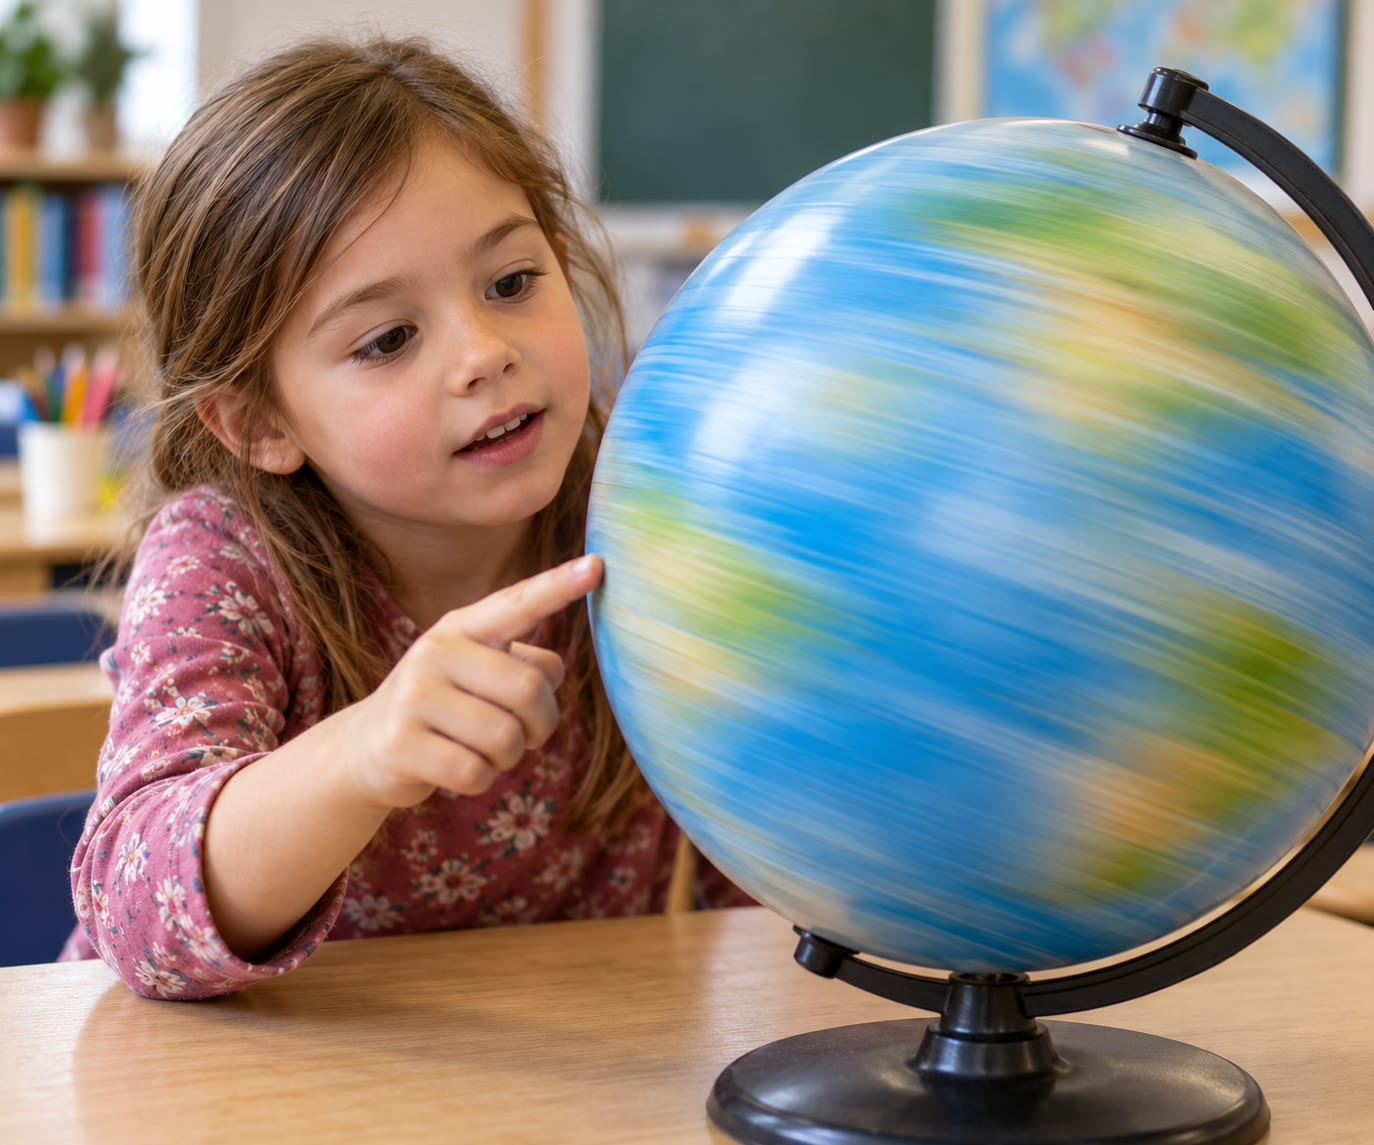
\includegraphics[width=0.6\linewidth]{images/book1/ai/g3-spinning-globe.jpg}

{\small A \omterm{def:g3:continents-and-oceans:globe}{globe} spinning on its stand: land and \omterm{def:g2:water-on-earth:ocean}{sea} go by under the
finger.}
\end{omfigure}

\begin{recall}
Most of the Earth is covered by \omterm{def:g2:water-on-earth:salt-fresh}{salt water}: about 71 squares out of 100 on
the grid of \cref{ch:g2:water-on-earth}. An \omterm{def:g2:water-on-earth:ocean}{ocean} is a very large stretch
of \omterm{def:g2:water-on-earth:salt-fresh}{salt water} between the land masses; a \omterm{def:g2:water-on-earth:ocean}{sea} is a smaller one, at the edge
of an \omterm{def:g2:water-on-earth:ocean}{ocean}. A \omterm{def:g2:drawing-to-map:map}{map} is a drawing of a place seen from above, made smaller
(\cref{ch:g2:drawing-to-map}). The physics books tell how the Earth turns on
itself once a day, which gives us day and night.
\end{recall}

\section{The globe, a small model of the round Earth}

The Earth is round, like a very big ball. We cannot see its shape from the
ground, because it is far too big: wherever we stand, the ground looks
flat. But astronauts who travelled far from the Earth saw it whole, a round
blue ball in the black sky (the photograph at the start of
\cref{ch:g2:water-on-earth}).

To see the whole Earth in a classroom, we make it small.

\begin{definition}[Globe]\label{def:g3:continents-and-oceans:globe}
A \emph{globe}\index{globe} is a model of the Earth: a ball on which the
land and the \omterm{def:g2:water-on-earth:ocean}{oceans} are drawn with the same shapes as on the real Earth,
only very much smaller.
\end{definition}

A \omterm{def:g3:continents-and-oceans:globe}{globe} is the best picture of the Earth, because it has the right shape:
round. But like the real Earth, we can only ever see one half of it at a
time. To see the other half, we turn it round.

\begin{omfigure}
\begin{tikzpicture}
\begin{axis}[name=atl, hide axis, axis equal image, scale only axis,
    width=6.2cm, xmin=-1.05, xmax=1.05, ymin=-1.05, ymax=1.05, clip=false]
  \fill[omSea] (axis cs:0,0) circle[radius=1];
  \addplot[fill=omHypsLandA!85!black, draw=black!45, line width=0.2pt]
    table {figdata/out/grade-3-globe-atlantic-land.dat};
  \addplot[black!60, dashed, line width=0.5pt]
    table {figdata/out/grade-3-globe-atlantic-equator.dat};
  \addplot[only marks, mark=*, mark size=1.4pt, black]
    table[x=x, y=y] {figdata/out/grade-3-globe-atlantic-poles.dat};
  \addplot[only marks, mark=none, nodes near coords, point meta=explicit symbolic,
    nodes near coords style={font=\scriptsize, anchor=center, fill=white, fill opacity=0.7, text opacity=1, inner sep=1pt, rounded corners=1pt}]
    table[x=x, y=y, meta=name] {figdata/out/grade-3-globe-atlantic-labels.dat};
  \draw[black!70, line width=0.8pt] (axis cs:0,0) circle[radius=1];
  \node[font=\scriptsize, anchor=south] at (axis cs:0,0.97) {North Pole};
\end{axis}
\begin{axis}[at={(atl.east)}, anchor=west, xshift=0.6cm, hide axis,
    axis equal image, scale only axis,
    width=6.2cm, xmin=-1.05, xmax=1.05, ymin=-1.05, ymax=1.05, clip=false]
  \fill[omSea] (axis cs:0,0) circle[radius=1];
  \addplot[fill=omHypsLandA!85!black, draw=black!45, line width=0.2pt]
    table {figdata/out/grade-3-globe-pacific-land.dat};
  \addplot[black!60, dashed, line width=0.5pt]
    table {figdata/out/grade-3-globe-pacific-equator.dat};
  \addplot[only marks, mark=none, nodes near coords, point meta=explicit symbolic,
    nodes near coords style={font=\scriptsize, anchor=center, fill=white, fill opacity=0.7, text opacity=1, inner sep=1pt, rounded corners=1pt}]
    table[x=x, y=y, meta=name] {figdata/out/grade-3-globe-pacific-labels.dat};
  \draw[black!70, line width=0.8pt] (axis cs:0,0) circle[radius=1];
\end{axis}
\end{tikzpicture}

{\small The \omterm{def:g3:continents-and-oceans:globe}{globe} seen from two sides. Left: the side of the Atlantic
\omterm{def:g2:water-on-earth:ocean}{Ocean}, with the Americas, Europe and Africa. Right: the other side, the
Pacific \omterm{def:g2:water-on-earth:ocean}{Ocean}, with Australia at its edge. The dashed line is the \omterm{def:g3:continents-and-oceans:equator}{equator}.
Coastlines: Natural Earth (public domain).}
\label{fig:g3:continents-and-oceans:globes}
% ledger: data:ne-land
\end{omfigure}

\begin{remark}[Two very different halves]\label{rem:g3:continents-and-oceans:halves}
Look at the two pictures. On the left, land covers about 4 parts of the
picture out of 10. On the right, only about 1 part out of 10: the Pacific
side of the Earth is almost all water. If Lena's finger stops on that side
of the \omterm{def:g3:continents-and-oceans:globe}{globe}, it will nearly always land on the \omterm{def:g2:water-on-earth:ocean}{sea}.
\end{remark}

\section{The equator, the poles and the two hemispheres}

A \omterm{def:g3:continents-and-oceans:globe}{globe} turns on a rod that goes right through it, from top to bottom.
The real Earth has no rod, but it also turns round a line through its
middle. The two places where that line comes out of the Earth have names.

\begin{definition}[Pole]\label{def:g3:continents-and-oceans:poles}
The \emph{North Pole}\index{North Pole} and the \emph{South
Pole}\index{South Pole} are the two points at the very top and the very
bottom of the Earth, where the line the Earth turns round comes out. Each
of them is a \emph{pole}\index{pole}. On a \omterm{def:g3:continents-and-oceans:globe}{globe}, the North Pole is at the
top.
\end{definition}

\begin{definition}[Equator and hemisphere]\label{def:g3:continents-and-oceans:equator}
The \emph{equator}\index{equator} is an imaginary line drawn all the way
round the Earth, exactly halfway between the \omterm{def:g3:continents-and-oceans:poles}{North Pole} and the \omterm{def:g3:continents-and-oceans:poles}{South Pole}.
It cuts the Earth into two halves, each called a
\emph{hemisphere}\index{hemisphere}: the \emph{northern
hemisphere}\index{northern hemisphere}, on the side of the \omterm{def:g3:continents-and-oceans:poles}{North Pole}, and
the \emph{southern hemisphere}\index{southern hemisphere}, on the side of
the \omterm{def:g3:continents-and-oceans:poles}{South Pole}.
\end{definition}

The \omterm{def:g3:continents-and-oceans:equator}{equator} is not painted on the ground: no one can see it on a beach or in
a forest. It is drawn on \omterm{def:g3:continents-and-oceans:globe}{globes} and on \omterm{def:g2:drawing-to-map:map}{maps} to help us find our way.

\begin{omfigure}
\begin{tikzpicture}[font=\small]
  % globe outline
  \fill[omSea!70] (0,0) circle (2.2);
  % northern hemisphere tinted
  \begin{scope}
    \clip (0,0) circle (2.2);
    \fill[yellow!25, opacity=0.8] (-2.3,0) -- (-2.3,2.3) -- (2.3,2.3) -- (2.3,0)
      arc[start angle=0, end angle=-180, x radius=2.3, y radius=0.45] -- cycle;
  \end{scope}
  \draw[black!70, line width=0.8pt] (0,0) circle (2.2);
  % equator: front half solid, back half dashed
  \draw[red!70!black, line width=1.2pt] (-2.2,0) arc[start angle=180, end angle=360, x radius=2.2, y radius=0.4];
  \draw[red!70!black, line width=0.8pt, dashed] (2.2,0) arc[start angle=0, end angle=180, x radius=2.2, y radius=0.4];
  % axis and poles
  \draw[black!60, line width=0.6pt] (0,2.2) -- (0,2.75);
  \draw[black!60, line width=0.6pt] (0,-2.2) -- (0,-2.75);
  \draw[black!60, line width=0.6pt, dotted] (0,2.2) -- (0,-2.2);
  \fill (0,2.2) circle (2.2pt);
  \fill (0,-2.2) circle (2.2pt);
  \node[anchor=west] at (0.15,2.6) {North Pole};
  \node[anchor=west] at (0.15,-2.6) {South Pole};
  % labels
  \node[anchor=west] at (2.6,0) {equator};
  \draw[black!60] (2.55,0) -- (2.05,-0.15);
  \node[anchor=west, align=left] at (2.6,1.4) {northern\\hemisphere};
  \draw[black!60] (2.55,1.4) -- (1.5,1.2);
  \node[anchor=west, align=left] at (2.6,-1.4) {southern\\hemisphere};
  \draw[black!60] (2.55,-1.4) -- (1.5,-1.2);
\end{tikzpicture}

{\small The \omterm{def:g3:continents-and-oceans:equator}{equator} cuts the Earth into two \omterm{def:g3:continents-and-oceans:equator}{hemispheres}. The \omterm{def:g3:continents-and-oceans:equator}{northern
hemisphere} (tinted) is on the side of the \omterm{def:g3:continents-and-oceans:poles}{North Pole}, the \omterm{def:g3:continents-and-oceans:equator}{southern
hemisphere} on the side of the \omterm{def:g3:continents-and-oceans:poles}{South Pole}.}
\label{fig:g3:continents-and-oceans:hemispheres}
\end{omfigure}

\begin{example}[Hot near the equator, cold near the poles]\label{ex:g3:continents-and-oceans:hot-cold}
The lands near the \omterm{def:g3:continents-and-oceans:equator}{equator} are hot all the year round: that is where the
great rainforests grow. The lands near the \omterm{def:g3:continents-and-oceans:poles}{poles} are cold all the year
round, and much of them is covered by ice. You will learn in a later year
why this is so; for now, remember: the closer to a \omterm{def:g3:continents-and-oceans:poles}{pole}, the colder.
\end{example}

\section{Seven continents and five oceans}

On a \omterm{def:g3:continents-and-oceans:globe}{globe}, the land is not spread out in little pieces everywhere. Most of
it is gathered in a few very large masses.

\begin{definition}[Continent]\label{def:g3:continents-and-oceans:continent}
A \emph{continent}\index{continent} is one of the very large masses of land
on the Earth, together with the islands close to it.
\end{definition}

People most often count seven \omterm{def:g3:continents-and-oceans:continent}{continents}. From the largest to the smallest
they are: Asia, Africa, North America, South America, Antarctica, Europe
and Australia.
% ledger: natgeo:seven-continents

\begin{center}\small
\begin{tabular}{rlll}
\hline
Size & \omterm{def:g3:continents-and-oceans:continent}{Continent} & \omterm{def:g3:continents-and-oceans:equator}{Hemisphere} & A word about it \\
\hline
1 & Asia & mostly northern & the largest \\
2 & Africa & both & the \omterm{def:g3:continents-and-oceans:equator}{equator} crosses its middle \\
3 & North America & northern & reaches far to the north \\
4 & South America & mostly southern & the \omterm{def:g3:continents-and-oceans:equator}{equator} crosses its north \\
5 & Antarctica & southern & around the \omterm{def:g3:continents-and-oceans:poles}{South Pole}, under ice \\
6 & Europe & northern & joined to Asia on its east side \\
7 & Australia & southern & the smallest \\
\hline
\end{tabular}
\end{center}

\begin{remark}[Where does one continent end?]\label{rem:g3:continents-and-oceans:where}
Some \omterm{def:g3:continents-and-oceans:continent}{continents} are surrounded by \omterm{def:g2:water-on-earth:ocean}{sea} on every side, like Australia or
Antarctica. Others touch: Europe and Asia are one single mass of land, and
people chose where to draw the line between them. That is why some people
count six \omterm{def:g3:continents-and-oceans:continent}{continents}, or even fewer.
\end{remark}

Between the \omterm{def:g3:continents-and-oceans:continent}{continents} lie the \omterm{def:g2:water-on-earth:ocean}{oceans}. There are five of them. The largest
is the \emph{Pacific \omterm{def:g2:water-on-earth:ocean}{Ocean}}; then come the \emph{Atlantic \omterm{def:g2:water-on-earth:ocean}{Ocean}}, the
\emph{Indian \omterm{def:g2:water-on-earth:ocean}{Ocean}}, the \emph{Southern \omterm{def:g2:water-on-earth:ocean}{Ocean}} around Antarctica, and the
smallest, the \emph{Arctic \omterm{def:g2:water-on-earth:ocean}{Ocean}} around the \omterm{def:g3:continents-and-oceans:poles}{North Pole}. For a long time
people counted only four; today most countries count the Southern \omterm{def:g2:water-on-earth:ocean}{Ocean} as
the fifth.
% ledger: nos:five-oceans, nos:pacific-largest, oer:arctic-smallest

\begin{example}[How big is the Pacific?]\label{ex:g3:continents-and-oceans:pacific}
The Pacific \omterm{def:g2:water-on-earth:ocean}{Ocean} is so big that all the \omterm{def:g3:continents-and-oceans:continent}{continents} put together could fit
inside it. It holds more than half of all the \omterm{def:g2:water-on-earth:ocean}{ocean} water on Earth. That is
why the right-hand \omterm{def:g3:continents-and-oceans:globe}{globe} in the first section of this chapter looks almost
all blue.
% ledger: nos:pacific-largest
\end{example}

\begin{method}[Naming the ocean between two continents]\label{met:g3:continents-and-oceans:between}
To find which \omterm{def:g2:water-on-earth:ocean}{ocean} lies between two \omterm{def:g3:continents-and-oceans:continent}{continents}, put a finger on each of
them on the \omterm{def:g3:continents-and-oceans:globe}{globe}, and turn the \omterm{def:g3:continents-and-oceans:globe}{globe} so that you can see both. The \omterm{def:g2:water-on-earth:ocean}{ocean}
your eye crosses to go from one finger to the other is the one between them.
On a \omterm{def:g3:continents-and-oceans:globe}{globe} there are often two ways round: take the shorter one.
\end{method}

\begin{example}[Africa and Australia]\label{ex:g3:continents-and-oceans:africa-australia}
Going from Africa east towards Australia, we cross the Indian \omterm{def:g2:water-on-earth:ocean}{Ocean}. Going
from Europe west to North America, we cross the Atlantic \omterm{def:g2:water-on-earth:ocean}{Ocean}. Going from
Asia east to North America, we cross the Pacific \omterm{def:g2:water-on-earth:ocean}{Ocean}.
\end{example}

\section{A world map is a flattened globe}

A \omterm{def:g3:continents-and-oceans:globe}{globe} is round, so it is not easy to carry, and we can never see all of
it at once. A \omterm{def:g2:drawing-to-map:map}{map} on a sheet of paper shows the whole Earth in one look.

\begin{definition}[World map]\label{def:g3:continents-and-oceans:world-map}
A \emph{world map}\index{world map} is a \omterm{def:g2:drawing-to-map:map}{map} of the whole Earth drawn flat
on a sheet of paper or on a screen, with all the \omterm{def:g3:continents-and-oceans:continent}{continents} and all the
\omterm{def:g2:water-on-earth:ocean}{oceans} in one picture.
\end{definition}

\begin{omfigure}
\begin{tikzpicture}
\begin{axis}[ommap, width=\linewidth, xtick=\empty, ytick={0},
    yticklabels={equator}, grid=none, clip=true]
  \addplot[fill=omHypsLandA!85!black, draw=black!45, line width=0.2pt]
    table {figdata/out/shared-geo-land.dat};
  \draw[black!60, dashed, line width=0.5pt] (axis cs:-180,0) -- (axis cs:180,0);
  \begin{scope}[every node/.style={font=\scriptsize, align=center}]
    \node at (axis cs:-102,47) {North\\America};
    \node at (axis cs:-60,-12) {South\\America};
    \node at (axis cs:17,52) {Europe};
    \node at (axis cs:20,6) {Africa};
    \node at (axis cs:92,48) {Asia};
    \node at (axis cs:134,-24) {Australia};
    \node at (axis cs:40,-80) {Antarctica};
  \end{scope}
  \begin{scope}[every node/.style={font=\scriptsize\itshape, align=center, text=omSea!35!black}]
    \node at (axis cs:-145,8) {Pacific\\Ocean};
    \node at (axis cs:165,12) {Pacific\\Ocean};
    \node at (axis cs:-38,22) {Atlantic\\Ocean};
    \node at (axis cs:-15,-25) {Atlantic\\Ocean};
    \node at (axis cs:78,-22) {Indian\\Ocean};
    \node at (axis cs:-115,-57) {Southern Ocean};
    \node at (axis cs:-150,79) {Arctic Ocean};
  \end{scope}
\end{axis}
\end{tikzpicture}

{\small A \omterm{def:g3:continents-and-oceans:world-map}{world map}. The \omterm{def:g3:continents-and-oceans:globe}{globe} has been cut along a line through the middle
of the Pacific \omterm{def:g2:water-on-earth:ocean}{Ocean} and stretched flat: the Pacific appears twice, on the
left and on the right edge. Antarctica, a round \omterm{def:g3:continents-and-oceans:continent}{continent} around the \omterm{def:g3:continents-and-oceans:poles}{South
Pole}, is stretched into a long band along the bottom.
Coastlines: Natural Earth (public domain).}
\label{fig:g3:continents-and-oceans:world-map}
% ledger: data:ne-land
\end{omfigure}

But there is a difficulty. Try to flatten the peel of an orange on a table:
it cannot lie flat without tearing or stretching. The same happens to the
surface of the \omterm{def:g3:continents-and-oceans:globe}{globe} when it is drawn flat. Every \omterm{def:g3:continents-and-oceans:world-map}{world map} tears the \omterm{def:g3:continents-and-oceans:globe}{globe}
somewhere, or stretches some places and squeezes others.

\begin{omfigure}
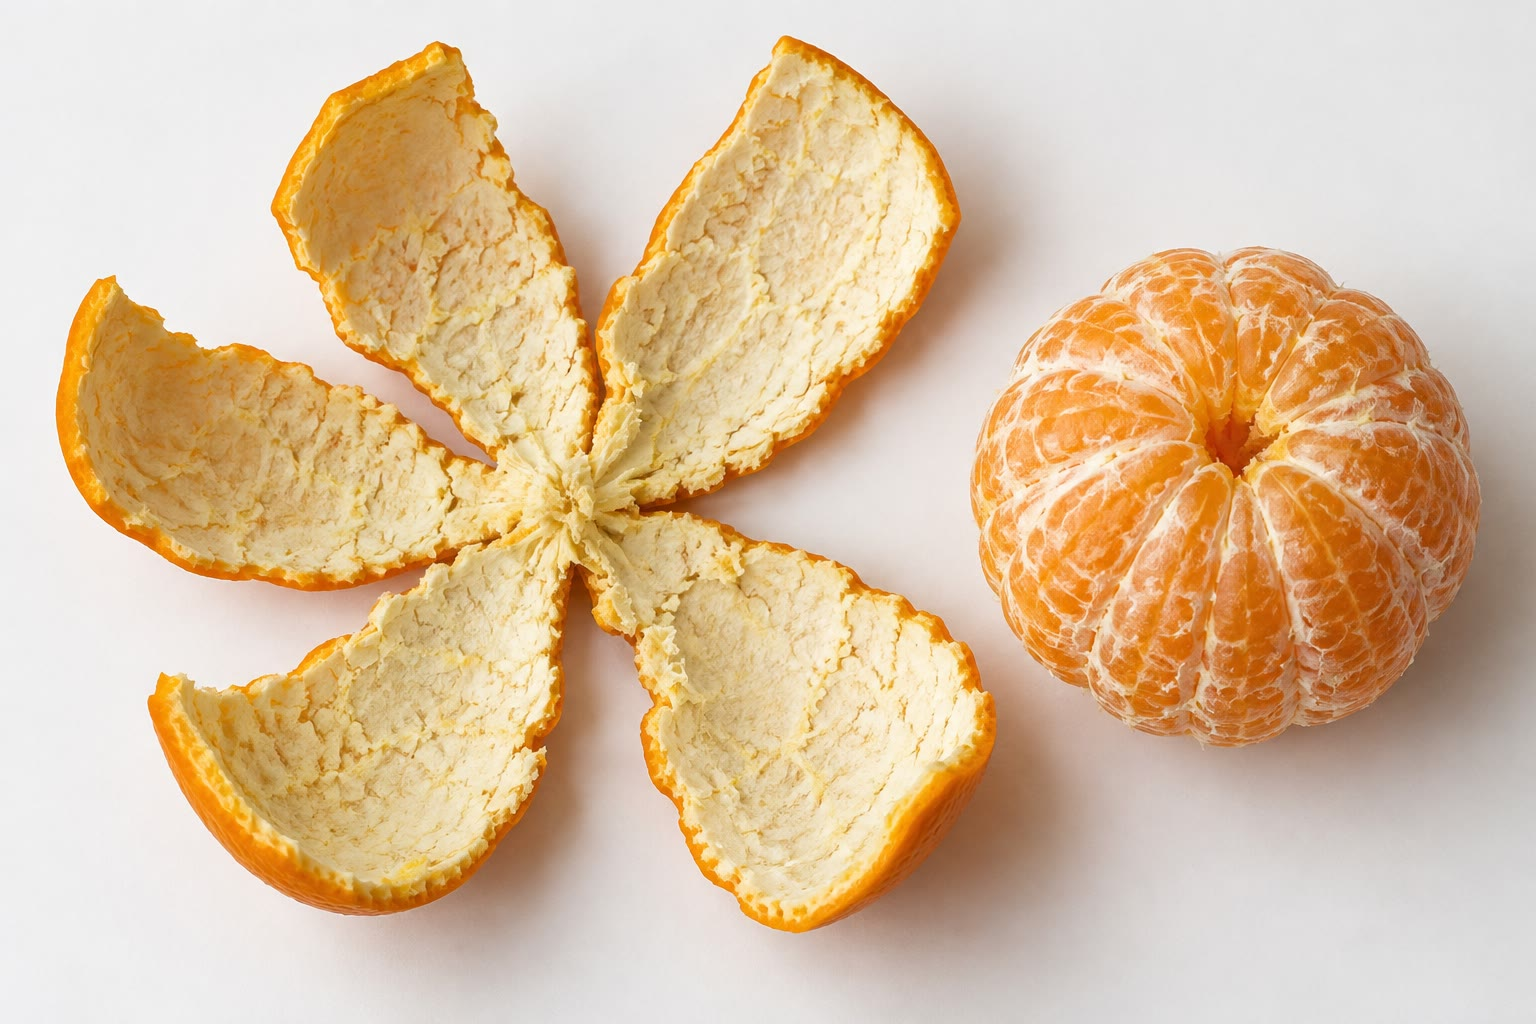
\includegraphics[width=0.4\linewidth]{images/book1/ai/g3-orange-peel.jpg}

{\small The peel of an orange cannot lie flat without tearing.}
\end{omfigure}

\begin{remark}[The map and the globe disagree]\label{rem:g3:continents-and-oceans:disagree}
On this \omterm{def:g3:continents-and-oceans:world-map}{world map}, Antarctica looks like one of the biggest \omterm{def:g3:continents-and-oceans:continent}{continents},
stretched along the whole bottom edge. On the \omterm{def:g3:continents-and-oceans:globe}{globe}, it is a round mass of
land, smaller than South America. Near the \omterm{def:g3:continents-and-oceans:poles}{poles}, a flat \omterm{def:g2:drawing-to-map:map}{map} stretches
the land a lot. Near the \omterm{def:g3:continents-and-oceans:equator}{equator}, it stretches it very little. When you
want to compare the size of two places far from the \omterm{def:g3:continents-and-oceans:equator}{equator}, the \omterm{def:g3:continents-and-oceans:globe}{globe}
tells the truth.
\end{remark}

\begin{method}[Reading a world map]\label{met:g3:continents-and-oceans:reading}
On a \omterm{def:g3:continents-and-oceans:world-map}{world map} like this one:
\begin{enumerate}
  \item north is at the top, south at the bottom; the \omterm{def:g3:continents-and-oceans:poles}{North Pole} is the
        whole top edge and the \omterm{def:g3:continents-and-oceans:poles}{South Pole} the whole bottom edge;
  \item the \omterm{def:g3:continents-and-oceans:equator}{equator} is the line across the middle: everything above it is in
        the \omterm{def:g3:continents-and-oceans:equator}{northern hemisphere}, everything below it in the \omterm{def:g3:continents-and-oceans:equator}{southern
        hemisphere};
  \item the left and the right edges are the same line on the \omterm{def:g3:continents-and-oceans:globe}{globe}: a
        ship that sails off the right edge comes back on the left.
\end{enumerate}
\end{method}

\section{Exercises}

\begin{exercise}[$\star$]\label{exo:g3:continents-and-oceans:1}
Name the seven \omterm{def:g3:continents-and-oceans:continent}{continents}. Which is the largest? Which is the smallest?
\end{exercise}

\begin{exercise}[$\star$]\label{exo:g3:continents-and-oceans:2}
Name the five \omterm{def:g2:water-on-earth:ocean}{oceans}. Which is the largest? Which is the smallest?
\end{exercise}

\begin{exercise}[$\star$]\label{exo:g3:continents-and-oceans:3}
Copy and fill in with ``\omterm{def:g3:continents-and-oceans:poles}{North Pole}'', ``\omterm{def:g3:continents-and-oceans:poles}{South Pole}'' or ``\omterm{def:g3:continents-and-oceans:equator}{equator}'': the
\dots{} is at the top of a \omterm{def:g3:continents-and-oceans:globe}{globe}; the \dots{} is at the bottom; the \dots{}
goes all the way round the middle.
\end{exercise}

\begin{exercise}[$\star$]\label{exo:g3:continents-and-oceans:4}
Northern or \omterm{def:g3:continents-and-oceans:equator}{southern hemisphere}? Europe; Australia; Antarctica; North
America.
\end{exercise}

\begin{exercise}[$\star$]\label{exo:g3:continents-and-oceans:5}
Which \omterm{def:g2:water-on-earth:ocean}{ocean} lies around the \omterm{def:g3:continents-and-oceans:poles}{North Pole}? Which \omterm{def:g2:water-on-earth:ocean}{ocean} lies around
Antarctica?
\end{exercise}

\begin{exercise}[$\star\star$]\label{exo:g3:continents-and-oceans:6}
Which \omterm{def:g2:water-on-earth:ocean}{ocean} do you cross to go from Africa to South America? From
Australia to South America, going east? From Africa to Australia?
\end{exercise}

\begin{exercise}[$\star\star$]\label{exo:g3:continents-and-oceans:7}
Sam lives in a country where it is hot all the year round. Bo lives on a
research station where it is freezing all the year round. One of them lives
near the \omterm{def:g3:continents-and-oceans:equator}{equator}, the other near a \omterm{def:g3:continents-and-oceans:poles}{pole}. Who lives where?
\end{exercise}

\begin{exercise}[$\star\star$]\label{exo:g3:continents-and-oceans:8}
Lena spins the \omterm{def:g3:continents-and-oceans:globe}{globe} 10 times. Her finger lands on the \omterm{def:g2:water-on-earth:ocean}{sea} 7 times. How
many times does it land on the land? Is this what you expected? Why?
\end{exercise}

\begin{exercise}[$\star\star$]\label{exo:g3:continents-and-oceans:9}
On the \omterm{def:g3:continents-and-oceans:world-map}{world map} on page~\pageref{fig:g3:continents-and-oceans:world-map}, the
Pacific \omterm{def:g2:water-on-earth:ocean}{Ocean} appears twice. Why? Does the real Earth have two Pacific
\omterm{def:g2:water-on-earth:ocean}{Oceans}?
\end{exercise}

\begin{exercise}[$\star\star\star$]\label{exo:g3:continents-and-oceans:10}
Tom says: ``On the \omterm{def:g3:continents-and-oceans:world-map}{world map}, Antarctica is longer than Asia, so Antarctica
is the biggest \omterm{def:g3:continents-and-oceans:continent}{continent}.'' Is Tom right? Use the list of the \omterm{def:g3:continents-and-oceans:continent}{continents}
from the largest to the smallest, and say why the \omterm{def:g3:continents-and-oceans:world-map}{world map} fools him.
\end{exercise}
